\chapter{PHP}
\label{php}\index{PHP}

PHP~\cite{php-in-action} is a server-side web scripting language. In its current version, it is object-oriented and dynamically typed. However, it provides some minimal type safety using type hinting, i.e., function parameters can be typed using class names or ``array'',  and \texttt{@var} annotations (which are not evaluated on execution). PHP provides lots of powerful built-in functions for cryptography, string handling, ZIP handling, networking, XML, and more.

\section{Challenges in static analysis for PHP}

In PHP, it is possible to use variables for variable names (which is called ``variable variables'')\index{variable variables}, field names, class names or for the inclusion of other classes. This practically is the same as multiple pointers in C++, and poses a problem for static analysis~\cite{tamper-resistance} that forces static analysis to fall back on approximations.

For example, the following constructs are possible, making static analysis a lot harder than e.g. for Java:

\begin{phpcode}
// bar contains the name of the class to instantiate.
$foo = new $bar();

// foo contains the name of the variable that gets assigned a 1.
$$foo = 1;
\end{phpcode}

\index{require\_once}
\begin{phpcode}
// classFile includes the path of the class file to include.
require_once($classFile);

// To correctly resolve this include, a scanner would need to parse how
// t3lib_extMgm::extPath creates paths.
require_once(t3lib_extMgm::extPath('seminars') .
  'pi2/class.tx_seminars_pi2.php');

// Depending on the value of classFlavor, different version of the same
// class will be used. This results in runtime class resolution.
switch ($classFlavor) {
  case FLAVOR_ORANGE:
    require_once('Orange.php');
    break;
  case FLAVOR_VANILLA:
    require_once('Vanilla.php');
    break;
  default;
    require_once('Default.php');
    break;
}
$bar = new MyClass();
\end{phpcode}.

\index{autoloading}\index{autoloader|see{autoloading}}
\begin{phpcode}
// The class file for this class has not been included and will be
// implictly loaded on-demand by the autoloader.
$container = new SmartContainer();
\end{phpcode}

In addition, type-hinted parameters can be overwritten within a function:\index{type hinting}

\begin{phpcode}
protected function foo(array $bar) {
  if (empty($bar)) {
    // bar changes its type from an array to an integer.
    $bar = 42;
  }
}
\end{phpcode}

\section{Variables, references and aliases}

To be able to conduct alias analysis for PHP, it is important to fully understand how variables and references in PHP work. This section covers this, including the implementation details of variables in PHP and the various types of references that are possible in PHP.


\subsection{Variables, ZVALs and reference counting}

Variables in PHP are assigned by value by default~\cite{php-manual-variables} and internally stored in a structure called \emph{ZVAL}.\index{ZVAL}\index{PHP variables}\index{variables} In one of the C header files~\cite{php-src-api-headers} in the PHP source code, the structure looks like this:

\begin{ccode}
struct _zval_struct {
  /* Variable information */
  zvalue_value value;       /* value */
  zend_uint refcount__gc;
  zend_uchar type;          /* active type */
  zend_uchar is_ref__gc;
};

typedef union _zvalue_value {
  long lval;     /* long value */
  double dval;   /* double value */
  struct {
    char *val;
    int len;
  } str;
  HashTable *ht;  /* hash table value */
  zend_object_value obj;
} zvalue_value;
\end{ccode}

So a variable basically consists of a name (which is stored outside the ZVAL structure~\cite{php-extensions-zval}), a type, a value, and a reference counter.\index{reference counting}

\paragraph{Note:} This applies to basic data types like integers, strings or floats. For objects, things are a bit more complicated (see below).

Let's assume we have the following code:

\begin{phpcode}
$x = 42;
xdebug_debug_zval('x');
\end{phpcode}

The command \texttt{xdebug\_debug\_zval} from the Xdebug PHP extension~\cite{xdebug-functions} outputs detailed information on the variable:

\begin{textcode}
x: (refcount=1, is_ref=0)=42
\end{textcode}

\begin{figure}[!h]
  \begin{center}
    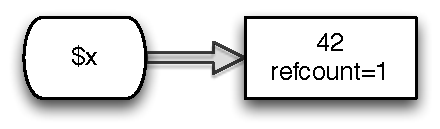
\includegraphics[scale=0.8]{images/x_42}
    \caption{a simple variable}
    \label{fig:simple-variable}
  \end{center}
\end{figure}

The reference count is used both by the garbage collector as well as to save memory by using a copy-on-write strategy.~\cite{php-manual-reference-counting}\index{copy-on-write}

\begin{phpcode}
$x = 42;
$y = $x;
xdebug_debug_zval('x');
xdebug_debug_zval('y');
\end{phpcode}

This code leads to both variables pointing to the exact same ZVAL, just by different names:

\begin{textcode}
x: (refcount=2, is_ref=0)=42
y: (refcount=2, is_ref=0)=42
\end{textcode}

\begin{figure}[!h]
  \begin{center}
    \includegraphics[scale=0.8]{images/x_y_42}
    \caption{two variables sharing the same ZVAL via copy-on-write}
    \label{fig:copy-on-write-variable}
  \end{center}
\end{figure}

When one of the variables is unset, the unset variable gets removed from the symbol table\index{symbol table} of the current scope, the reference counter is decreased again:

\begin{phpcode}
unset($y);
xdebug_debug_zval('x');
\end{phpcode}

\begin{textcode}
x: (refcount=1, is_ref=0)=42
\end{textcode}

When one of the variables is overwritten later, PHP creates a new ZVAL for the new value and decreases the reference count of the first ZVAL:

\begin{phpcode}
$x = 3;
xdebug_debug_zval('x');
xdebug_debug_zval('y');
\end{phpcode}

\begin{textcode}
x: (refcount=1, is_ref=0)=3
y: (refcount=1, is_ref=0)=42
\end{textcode}

\paragraph{Note:} \texttt{xdebug\_debug\_zval} will never display a \texttt{refcount} of zero for a variable because \texttt{xdebug\_debug\_zval} cannot display variables that have been unset (and that, by definition, do not exist at that point anymore).

\paragraph{Note:} To get PHP to actually use copy-on-write, it is necessary to directly copy the value of one variable to another variable. Just assigning variables the same value will not lead to both variables sharing one ZVAL. This is different from the way the Java virtual machine handles strings (in order to conserve memory).~\cite[chapter~2]{jvm-spec}\index{Java}\index{strings in Java}


\subsection{References}

References in PHP are two variables pointing to the same ZVAL. The PHP manual takes particular care to make the difference to C pointers clear:~\cite{php-manual-what-references-are}\cite{php-manual-what-references-are-not}\index{references}\index{C/C++ pointers}\index{pointers in C/C++}

There are several ways in which it is possible to create references in PHP: Assigning by reference, passing by reference and returning references.~\cite{php-manual-references}

\begin{quote}
References in PHP are a means to access the same variable content by different names. They are not like C pointers; for instance, you cannot perform pointer arithmetic using them, they are not actual memory addresses, and so on.
\end{quote}

\subsubsection{Assigning by reference}
\index{assigning by reference}

\paragraph{Creating references:}

References from one variable to another are set using the \texttt{=\&} operator.~\cite[page 129]{wenz-php53}\cite{php-manual-what-references-do} After this, both variables refer to the same ZVAL (instead of one variable pointing to the other), and it is not possible to distinguish between the referenced variable and the referencing variable anymore. Changing the value of one of the variables then changes the value in existing the ZVAL (and thus for both variables). However, it does \emph{not} create a new ZVAL.

The corresponding ZVAL is marked with with \texttt{is\_ref=1} (which is a 0/1 boolean flag, not a counter), and the reference count is increased:

\begin{phpcode}
$a1 = 'foo';
$a2 =& $a1;
$a1 = 'bar';
xdebug_debug_zval('a1');
xdebug_debug_zval('a2');
\end{phpcode}

\begin{textcode}
a1: (refcount=2, is_ref=1)='bar'
a2: (refcount=2, is_ref=1)='bar'
\end{textcode}

\begin{figure}[!h]
  \begin{center}
    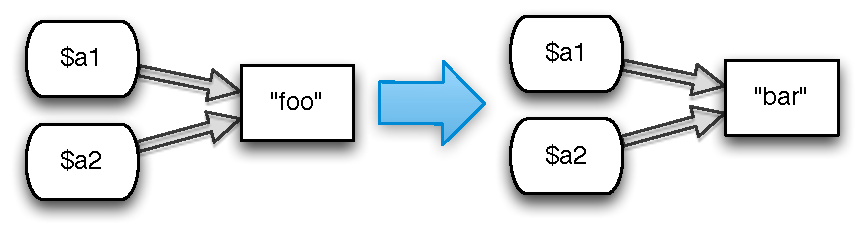
\includegraphics[scale=0.8]{images/a1_a2}
    \caption{two variables sharing the same ZVAL via a reference}
    \label{fig:simple-reference}
  \end{center}
\end{figure}


The same mechanism also applies when the content of a variable is copied to a variable that is a reference. In the following example, the content of \texttt{\$q3} is copied to \texttt{\$q2}, thus also changing the value of \texttt{\$q1} as both \texttt{\$q1} and \texttt{\$q2} are references to the same ZVAL:

\begin{phpcode}
$q1 = 'foo';
$q2 =& $q1;

$q3 = 'bar';
$q2 = $q3;
xdebug_debug_zval('q1');
xdebug_debug_zval('q2');
\end{phpcode}

\begin{textcode}
q1: (refcount=2, is_ref=1)='bar'
q2: (refcount=2, is_ref=1)='bar'
\end{textcode}

\begin{figure}[!h]
  \begin{center}
    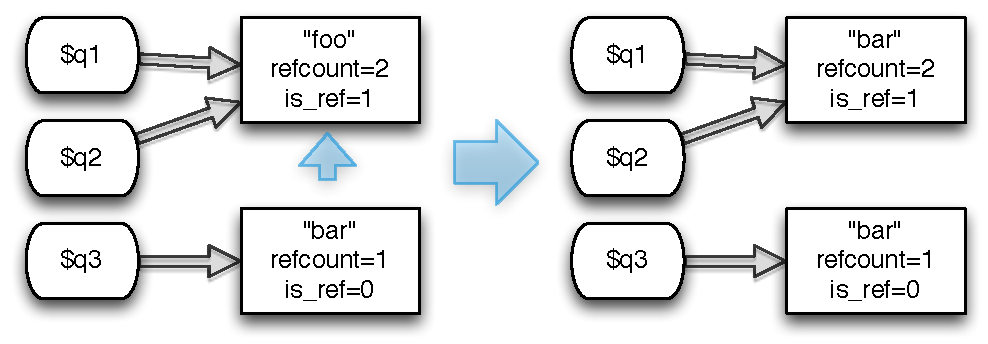
\includegraphics[scale=0.8]{images/q1_q2_q3}
    \caption{copying the value of one variable to two reference variables}
    \label{fig:copying-value-to-reference}
  \end{center}
\end{figure}



However, when a variable that is a reference to some variable is changed to be a reference to a different variablem, this changes only the entry in the symbol table, not the ZVAL. In the following exampled, \texttt{\$p2} is a reference to \texttt{\$p1} and then gets changed to be a reference to \texttt{\$p3}. \texttt{\$p1} stays unchanged as the corresponding ZVAL is not modified.

\begin{phpcode}
$p1 = 'foo';
$p2 =& $p1;

$p3 = 'bar';
$p2 =& $p3;
xdebug_debug_zval('p1');
xdebug_debug_zval('p2');
\end{phpcode}

\begin{textcode}
p1: (refcount=1, is_ref=0)='foo'
p2: (refcount=2, is_ref=1)='bar'
\end{textcode}

\begin{figure}[!h]
  \begin{center}
    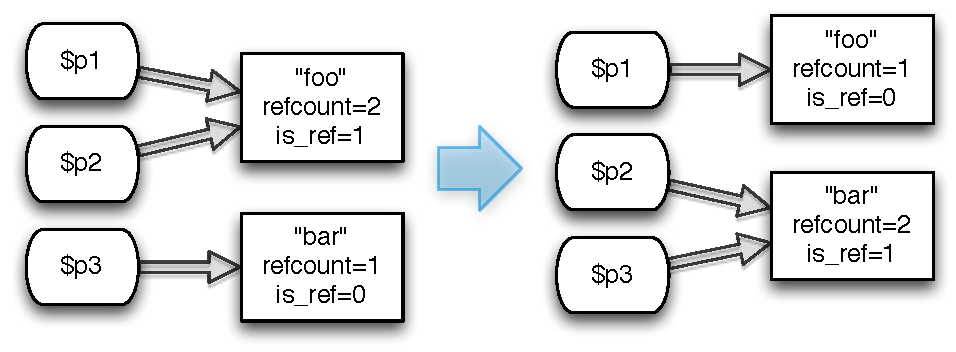
\includegraphics[scale=0.8]{images/p1_p2_p3}
    \caption{changing a reference variable from one ZVAL to another ZVAL}
    \label{fig:changing-references}
  \end{center}
\end{figure}




\paragraph{Dropping references and reference counting:}
\index{reference counting}

When a variable that is a reference is unset, PHP removes the variable from the symbol table of the current scope (i.\,e., it cuts the connection between the variable name and the ZVAL) and decreases the reference count. The ZVAL will not be destroyed (or be allowed for garbage collection) as long as the reference count is greater than zero.

There is a difference between cases where there are at least two references to the same ZVAL and cases where there is only one reference left. For at least two references, the ZVAL will still be marked as \texttt{is\_ref=1}:

\begin{phpcode}
$a1 = 'foo';
$a2 =& $a1;
$a3 =& $a1;
unset($a2);
xdebug_debug_zval('a1');
\end{phpcode}

\begin{textcode}
a1: (refcount=2, is_ref=1)='foo'
\end{textcode}

If there is only one reference to the ZVAL left, it will be marked as \texttt{is\_ref=0} (even if the variable that is left standing after all its fellows have been unset is not the original first variable):

\begin{phpcode}
$b1 = 'foo';
$b2 =& $b1;
unset($b1);
xdebug_debug_zval('b2');
\end{phpcode}

\begin{textcode}
b2: (refcount=1, is_ref=0)='foo'
\end{textcode}

\paragraph{Note:} References can only be created to variables\footnote{References to objects created with \texttt{new} in the same call are also possible. However, this usage of references has been deprecated in PHP 5.0.~\cite{php-manual-what-references-do}}, but not to literal values:

\begin{phpcode}
$answer =& 42;
\end{phpcode}

\begin{textcode}
PHP Parse error:  syntax error, unexpected '42' (T_LNUMBER) in
  /tmp/zval-test.php on line 2
\end{textcode}


\subsubsection{Returning by reference}
\index{returning by reference}

In PHP, functions (and thus also methods) normally return their return values by value. However, it is possible to change this so that the value is returned by reference:~\cite{php-manual-returning-reference}

\begin{phpcode}
class Foo {
  public $property = 0;

  public function &getProperty() {
    return $this->property;
  }
}

$foo = new Foo();
$property =& $foo->getProperty();
$property = 4;

xdebug_debug_zval('foo');
\end{phpcode}

\begin{textcode}
foo: (refcount=1, is_ref=0)=class Foo
  { public $property = (refcount=2, is_ref=1)=4 }
\end{textcode}

For returning by reference to actually work, both ampersand signs are necessary: the ampersand in the function declaration \texttt{function \&getProperty()} (so that the function returns the value by reference) as well as the ampersand when using the return value \texttt{\$property = \&\$foo->getProperty();} (so that \texttt{\$property} is assigned by reference, not by value.


\subsubsection{Passing by reference}
\index{passing by reference}

Variables can also be passed to functions (and methods) by reference. \cite{php-manual-passing-by-reference} This allows the function to change the value of the passed variable. (By default, function parameters are passed by value, not by reference.)

\begin{phpcode}
function changeParameter(&$parameter) {
  $parameter = 42;
}

$a = 5;
changeParameter($a);

xdebug_debug_zval('a');
\end{phpcode}

\begin{textcode}
a: (refcount=1, is_ref=0)=42
\end{textcode}


\subsection{References and objects}

Starting from PHP~5, objects are always passed kind of by reference:~\cite{php-manual-migration5-oop}

\begin{quote}
In PHP 5 there is a new Object Model. PHP's handling of objects has been completely rewritten, allowing for better performance and more features. In previous versions of PHP, objects were handled like primitive types (for instance integers and strings). The drawback of this method was that semantically the whole object was copied when a variable was assigned, or passed as a parameter to a method. In the new approach, objects are referenced by handle, and not by value (one can think of a handle as an object's identifier).
\end{quote}

The astute reader might have noticed the wording ``kind of by reference'' above. Actually, objects do not exactly work like references. Instead, variables that are object instances, the ZVAL contains a \emph{handle} (or object \emph{identifier}) for the object, not the object itself. So if variables (inderectly) point to the same object, they variables actually contains \emph{copies} of the indentifier.~\cite{php-manual-oop-references}

As long as the object is merely accessed, object variables work just like references:

\begin{phpcode}
$instance = new StdClass();
$instance->field = 'foo';

$instance2 = $instance;
$instance2->field = 'bar';

xdebug_debug_zval('instance');
xdebug_debug_zval('instance2');
\end{phpcode}

\begin{textcode}
instance: (refcount=2, is_ref=0)=class stdClass
  { public $field = (refcount=1, is_ref=0)='bar' }
instance2: (refcount=2, is_ref=0)=class stdClass
  { public $field = (refcount=1, is_ref=0)='bar' }
\end{textcode}

(In the output of \texttt{xdebug\_debug\_zval}, it unfortunately is not possible to see that the ZVALs only contain the object identifiers, not the object itself.)

\begin{figure}[!h]
  \begin{center}
    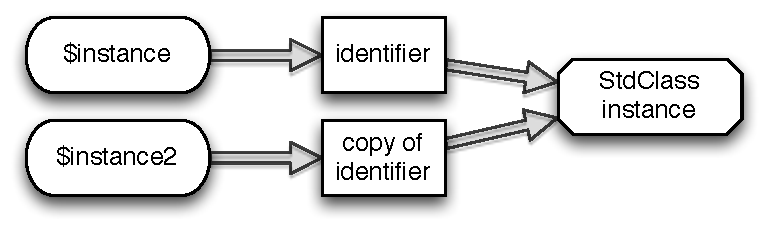
\includegraphics[scale=0.8]{images/instance_instance2}
    \caption{objects using the ZVAL for the object identifier/handle}
    \label{fig:objects}
  \end{center}
\end{figure}



However, if we start to use the object variables like real references and try to overwrite one object by setting the other object, the difference to real references becomes apparent:

\begin{phpcode}
$someInstance = new StdClass();
$someInstance->field = 'foo';

$instance2 = $instance;
$instance2 = 42;

xdebug_debug_zval('instance');
xdebug_debug_zval('instance2');
\end{phpcode}

\begin{textcode}
instance: (refcount=1, is_ref=0)=class stdClass
  { public $field = (refcount=1, is_ref=0)='bar' }
instance2: (refcount=1, is_ref=0)=42
\end{textcode}

\begin{figure}[!h]
  \begin{center}
    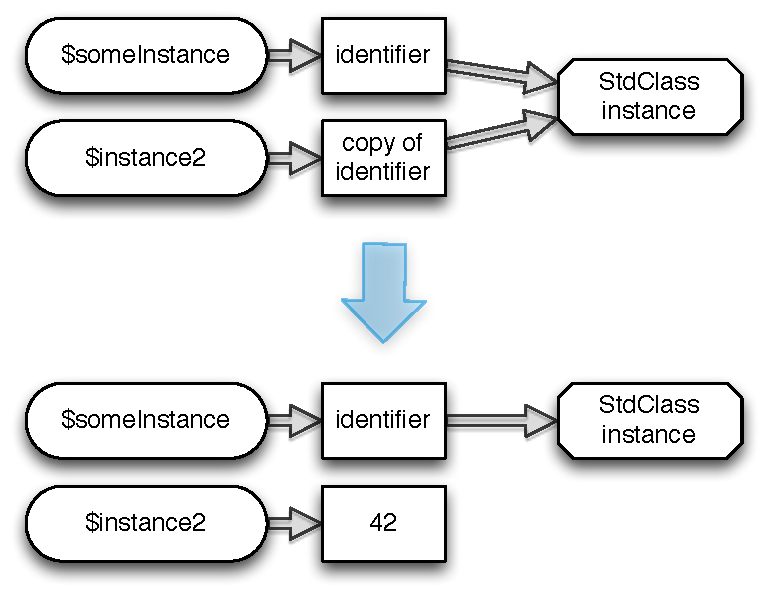
\includegraphics[scale=0.8]{images/someInstance_instance2}
    \caption{object handle variables that do not work like real references}
    \label{fig:false-object-references}
  \end{center}
\end{figure}

However, object variables can also be used as real references (again by using the ampersand \texttt{\&} operator):

\begin{phpcode}
$someInstance = new StdClass();
$someInstance->field = 'foo';

$instanceReference =& $someInstance;
$instanceReference = 42;

xdebug_debug_zval('someInstance');
xdebug_debug_zval('instanceReference');
\end{phpcode}

\begin{textcode}
someInstance: (refcount=2, is_ref=1)=42
instanceReference: (refcount=2, is_ref=1)=42
\end{textcode}

\begin{figure}[!h]
  \begin{center}
    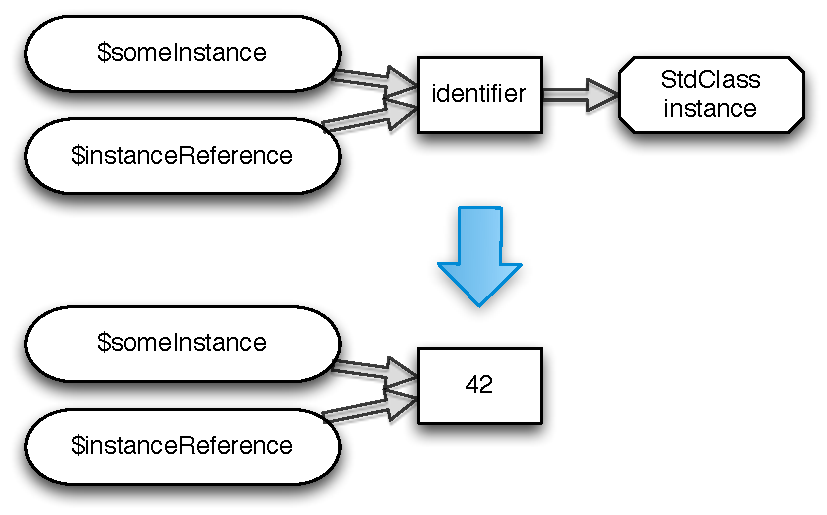
\includegraphics[scale=0.8]{images/someInstance_instanceReference}
    \caption{real object references}
    \label{fig:real-object-references}
  \end{center}
\end{figure}
